% DAFN - ROS 2 - Lecture 1: Middleware Fundamentals
% Roberto Masocco <roberto.masocco@uniroma2.it>
% March 6, 2022

\documentclass{beamer}

% Slides layout
\usepackage[
    title={Robot Operating System 2},
    subtitle={Lecture 1: Middleware Fundamentals},
    event={DAFN},
    author={Roberto Masocco},
    longauthor={Roberto Masocco},
    email={roberto.masocco@uniroma2.it},
    institute={Tor Vergata},
    longinstitute={University of Rome "Tor Vergata"},
    department={Department of Civil Engineering and Computer Science Engineering},
    researchgroup={Intelligent Systems Lab},
    date={April 27, 2022}
]{utvengbeamer}

% Code listings settings
\usepackage[nomath]{lmodern}
\definecolor{codegreen}{rgb}{0 0.5 0}
\definecolor{codered}{rgb}{1 0 0}
\definecolor{codeocher}{rgb}{0.8 0.47 0.13}
\usepackage{listings}
\lstdefinestyle{beamer}{
    basicstyle=\ttfamily\small,
    commentstyle=\color{codegreen},
    breakatwhitespace=false,
    captionpos=b,
    frame=lines,
    keepspaces=true,
    keywordstyle=\color{codered}\bfseries,
    numbers=left,
    numbersep=5pt,
    numberstyle=\footnotesize,
    showspaces=false,
    showstringspaces=false,
    showtabs=false,
    stringstyle=\color{codeocher},
    tabsize=2
}
\lstset{style=beamer}
\lstdefinelanguage{ros2msg}{
  alsoletter={[, ], _, /},
  morecomment=[l][\color{codegreen}]{\#},
  morekeywords={int64, uint32, string, uint8, uint8[], std_msgs/Header}
}

\usepackage{hyperref}

\begin{document}

% --- Title page ---
\frame{\titlepage}

% --- Table of contents ---
\begin{frame}
\frametitle{Roadmap}
\tableofcontents
\end{frame}

% --- Section 1 ---
% Section 1 - Middleware in robotics
% Roberto Masocco <roberto.masocco@uniroma2.it>
% March 13, 2022

% ### Middleware in robotics ###
\section{Middleware in robotics}
\graphicspath{{figs/section1/}}

% --- What is middleware? ---
\begin{frame}{What is middleware?}
	\begin{figure}
		\centering
		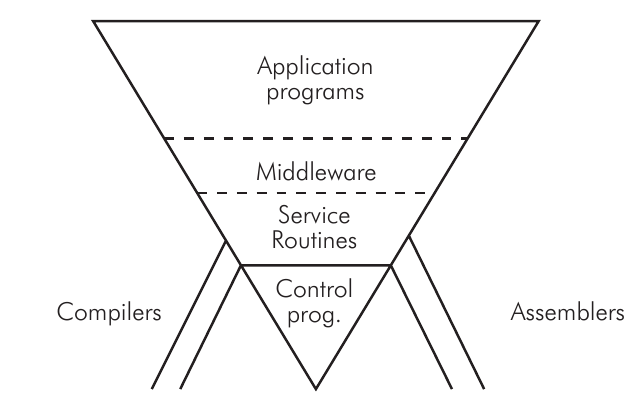
\includegraphics[width=.85\textwidth]{softwarePyramid.png}
		\caption{Software organization in a generic computer system}
		\label{fig:swpyramid}
	\end{figure}
\end{frame}
\begin{frame}{What is middleware?}
	\begin{block}{Definition of middleware}
		\justifying
		The term \textbf{middleware} identifies a kind of software that offers common services and functionalities to applications in addition to what an operating system usually does.
	\end{block}
	\justifying
	Middlewares are usually implemented as \textbg{libraries} that application programmers can use via appropriate \textbg{APIs}.
\end{frame}

% --- Middleware in robotics ---
\begin{frame}{Middleware in robotics}
	\justifying
	New problems arising when developing software for modern autonomous systems:
	\begin{itemize}
		\item integration of sophisticated hardware (not only microcontrollers!);
		\item software organization and maintenance;
		\item communication (involves both hardware and software!);
		\item debugging and testing.
	\end{itemize}
	\begin{block}{}
		\centering
		Middlewares can help to tackle and solve each one!
	\end{block}
\end{frame}

% --- Data Distribution Service ---
\begin{frame}{Data Distribution Service}
	\begin{block}{Definition of DDS}
		A DDS is a \textbf{publish-subscribe middleware} that handles communications between \textbf{real-time} systems and software over the network.
	\end{block}
	DDS implementations follow an open standard that defines:
	\begin{itemize}
		\item \textbg{serialization} and \textbg{deserialization} of data packets;
		\item automatic discovery of \textbg{DDS participants} (over \textbg{multicast-IP/UDP}) and transmission of data (over \textbg{unicast-IP/UDP});
		\item \textbg{security protocols} and cryptographic operations;
		\item enforcing of \textbg{Quality of Service} policies to organize transmissions (specifying things like \textbg{queue sizes}, \textbg{best-effort} or \textbg{reliable} transmissions...).
	\end{itemize}
	DDSs are currently used in automotive, aerospace, military...
\end{frame}
\begin{frame}{Data Distribution Service}
	\begin{figure}
		\centering
		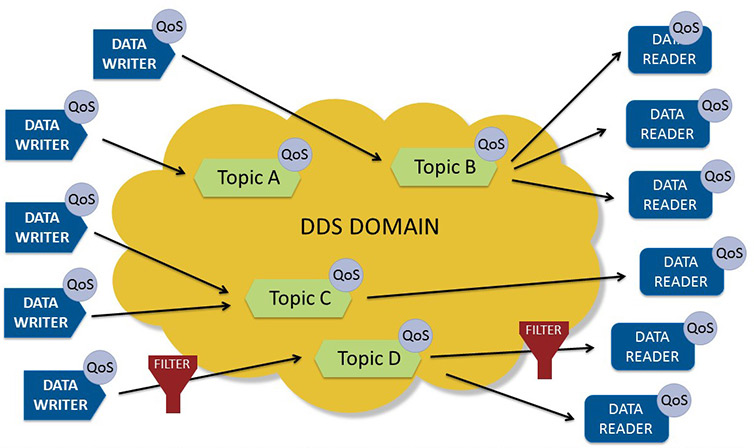
\includegraphics[width=.85\textwidth]{ddsDomain.jpg}
		\caption{Scheme of a DDS-based network}
		\label{fig:ddsdomain}
	\end{figure}
\end{frame}
\begin{frame}{Data Distribution Service}
	DDS participants can either \textbg{publish to} or \textbg{subscribe to} a \textbg{topic}.
	\begin{block}{Definition of DDS topic}
		A DDS topic is uniquely identified by three things:
		\begin{itemize}
			\item a \textbf{name}, i.e. a human-readable character string;
			\item an \textbf{interface}, i.e. a custom packet format that specifies what data is carried over it (e.g. strings, numbers, arrays...);
			\item a \textbf{QoS policy} that specifies how transmissions should be performed.
		\end{itemize}
	\end{block}
	\begin{block}{}
		\centering
		Changing even only one of the above results in a completely different topic!
	\end{block}
\end{frame}


% --- Section 2 ---
% Section 2 - ROS 2 Overview
% Roberto Masocco <roberto.masocco@uniroma2.it>
% March 13, 2022

% ### ROS 2 Overview ###
\section{ROS 2 Overview}
\graphicspath{{figs/section2/}}

% --- What is ROS 2? ---
\begin{frame}{What is ROS 2?}
\begin{columns}
    \column{.5\textwidth}
    \only<1>{
        \nolistindent ROS 2 is a \textbg{DDS-based}, \textbg{open-source} middleware for robotic applications. It allows developers to build and manage \textbg{distributed control architectures} made of many modules, usually referred to as \textbg{nodes}.
    }
    \only<2>{
        \nolistindent \nolistindent ROS 2 currently supports \textbg{C++} and \textbg{Python} for application programming, and runs natively on \textbg{Ubuntu Linux 20.04}.\\
        New versions are periodically released as \textbg{distributions}: the current LTS one is \textbg{Foxy Fitzroy} and the latest one today is \textbg{Galactic Geochelone}; the development version is \textbg{Rolling Ridley} and can only be compiled from source.
    }

    \column{.5\textwidth}
    \begin{figure}
        \centering
        
\includegraphics[width=.9\textwidth]{ros2Logo.jpg}
        \caption{ROS 2 logo}
        \label{fig:ros2logos}
    \end{figure}
\end{columns}
\end{frame}

% --- Main Features ---
\begin{frame}{Main Features}
As a middleware, it offers the following services to roboticists:
\begin{itemize}
    \item<1-> \textbg{three inter-process communication (IPC) paradigms}, easy to set up and based on the DDS;
    \item organization of software packages, allowing for \textbg{redistribution and code reuse}, thanks to the \textbg{colcon} package manager;
    \item<1-> module configuration tools: \textbg{node parameters} and \textbg{launch files};
    \item<1-> integrated \textbg{logging subsystem} (involves both console and log files);
    \item<1-> CLI \textbg{introspection tools} for debugging and testing;
    \item<1-> integration with \textbg{simulators} (e.g. Gazebo) and \textbg{data visualizers} (e.g. RViz);
    \item<2> and much more...
\end{itemize}
\end{frame}

% --- Flaws ---
\begin{frame}{Flaws}
\visible<1->{
    \begin{alertblock}{ROS 2 biggest flaws (as of today)}
        The main concerns arise when developing low-level stuff:
        \begin{itemize}
            \item the DDS layer is almost completely abstracted, so some network configurations are impossible;
            \item the internal job scheduling algorithm (the \textbr{executor}) is \textbr{not suited for hard real-time applications}.
        \end{itemize}
    \end{alertblock}
}
\visible<2>{
    What to do when development gets to a really low level?
    \begin{itemize}
        \item Use \textbg{micro-ROS}: ROS 2 on microcontrollers and different communication interfaces.
        \item Hand off stuff to \textbg{microcontrollers}.
        \item Use something else.
    \end{itemize}
}
\end{frame}

% --- Job Executor ---
\begin{frame}{Job Executor}
TODO:
\begin{itemize}
    \item event-based explanation
    \item node jobs+executor+callback scheme
    \item "to be addressed in new upcoming releases+micro-ROS"
\end{itemize}
\end{frame}


% --- Section 3 ---
% Section 3 - Basic Communication
% Roberto Masocco <roberto.masocco@uniroma2.it>
% March 13, 2022

% ### Basic Communication ###
\section{Basic Communication}
\graphicspath{{figs/section3/}}

% --- ROS 2 Messages ---
\begin{frame}{ROS 2 Messages}
    \begin{block}{Definition of Message}
      A message is a \textbf{single DDS data packet} sent over a \textbf{topic}, from \textbf{publisher nodes} to \textbf{subscriber nodes}, with a specific \textbf{QoS policy}.
    \end{block}
    \begin{figure}
      \centering
      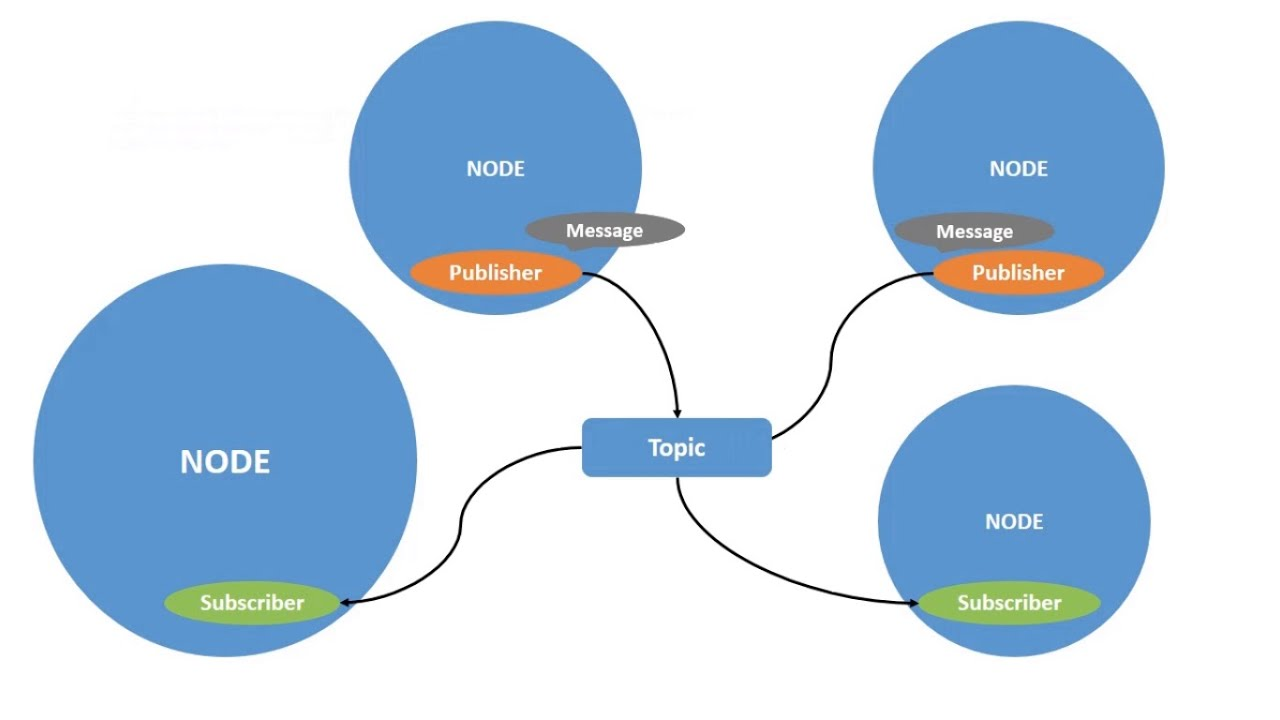
\includegraphics[scale=.19]{ros2Msg.jpg}
      \label{fig:msg}
      \caption{Example of a topic with multiple publisher and subscriber nodes}
    \end{figure}
\end{frame}

% --- Interface Files - Messages ---
\begin{frame}[fragile]{Interface Files - Messages}
Interface files format is specified by the DDS, with data types resolved to machine types according to the platform being used\footnote{\href{https://docs.ros.org/en/galactic/Concepts/About-ROS-Interfaces.html}{\color{blue}\underline{About ROS Interfaces}} (ROS 2 Galactic docs)}.\\
Things start very simply...

\begin{columns}
\column{.95\textwidth}
% Listing: std_msgs/msg/Int64 message definition
\begin{lstlisting}[language=ros2msg, caption=Definition of the \texttt{std\_msgs/msg/Int64} message]
int64 data
\end{lstlisting}

% Listing: std_msgs/msg/String message definition
\begin{lstlisting}[language=ros2msg, caption=Definition of the \texttt{std\_msgs/msg/String} message]
string data
\end{lstlisting}
\end{columns}

\end{frame}
\begin{frame}[fragile]{Interface Files - Messages}
... then escalate quickly!

\begin{columns}
\column{.95\textwidth}
% Listing: sensor_msgs/msg/Image
\begin{lstlisting}[language=ros2msg, caption=Definition of the \texttt{sensor\_msgs/msg/Image} composite message]
std_msgs/Header header

uint32 height
uint32 width

string encoding

uint8 is_bigendian
uint32 step
uint8[] data
\end{lstlisting}
\end{columns}

\end{frame}
\begin{frame}[fragile]{Interface Files - Messages}
Special values (i.e. constants) may be specified.

\begin{columns}
\column{.95\textwidth}
% Listing: message with constant
\begin{lstlisting}[language=ros2msg, caption=Definition of an example message with a constant value]
int64 MYNUM=1 # Must be of compatible type

int64 number
\end{lstlisting}
\end{columns}

They are not bound to any field and will appear as special selectable values in the generated C++/Python libraries.\\
ROS 2 adds its own guidelines\footnote{\href{https://github.com/IntelligentSystemsLabUTV/ros2-examples/blob/galactic/interfaces.md}{\color{blue}\underline{ros2-examples/interfaces.md}}}, and installed interfaces can be inspected with the \texttt{ros2 interface show} command.
\end{frame}

% --- Message Topics - Quality of Service ---
\begin{frame}{Message Topics - Quality of Service}
A \textbg{QoS policy}\footnote{\href{https://docs.ros.org/en/galactic/Concepts/About-Quality-of-Service-Settings.html}{\color{blue}\underline{About QoS Settings}} (ROS 2 Galactic docs)} for publishers/subscribers has the following attributes:
\begin{itemize}
  \item \textbg{History} (\emph{keep last N} or \emph{all})
  \item \textbg{Depth} (queue size \emph{N})
  \item \textbg{Reliability} (\emph{best-effort} or \emph{reliable}, default: reliable)
  \item \textbg{Durability} (publishers resend all messages to "late-joiners")
  \item Deadline
  \item \textbg{Lifespan} (message expiration date)
  \item Liveliness
  \item Lease Duration
\end{itemize}
Default \textbg{profiles} are available (e.g. \textbg{Sensor data}, \textbg{Service}...).
\end{frame}

% --- C++ Fundamentals ---
\begin{frame}[fragile]{C++ Fundamentals}
Dust off your C programming skills, then add:
\begin{block}{Object-Oriented Programming}
\begin{columns}
\column{.9\textwidth}
% Listing: C++ OOP example
\begin{lstlisting}[language=C++, caption=Example of definition of a C++ class]
class MyClass : public ParentClass
{
public:
  MyClass();
  // ...
protected:
  // ...
private:
  // ...
};
\end{lstlisting}
\end{columns}
\end{block}
\end{frame}
\begin{frame}[fragile]{C++ Fundamentals}
\begin{block}{Namespaces}
Subdivision of the global namespace to avoid naming collisions between multiple libraries, resolved with the \texttt{::} operator.

\begin{columns}
\column{.9\textwidth}
% Listings: C++ namespaces usage example
\begin{lstlisting}[language=C++, caption=Example of namespaces usage]
MyLib::foo();
MyClass::foo();
// Completely different names for the compiler!
\end{lstlisting}
\end{columns}

Names may become very long, so usually they are hidden with \texttt{typedef}.
\end{block}
\end{frame}
\begin{frame}[fragile]{C++ Fundamentals}
\begin{block}{Templates}
Classes or functions whose implementation depends on some data type. When instantiated or called with a specific type, the corresponding code is generated by the compiler.

\begin{columns}
\column{.9\textwidth}
% Listings: C++ template objects example
\begin{lstlisting}[language=C++, caption=Example of objects of the template class \texttt{std::vector}]
std::vector<int> int_vector;
std::vector<double> double_vector;
\end{lstlisting}
\end{columns}

These too make names very long, so are usually typedef'd.
\end{block}
\end{frame}
\begin{frame}[fragile]{C++ Fundamentals}
\begin{block}{Shared Pointers}
A kind of \textbf{smart pointer} (there are also \texttt{unique} and \texttt{weak}) that also holds an \textbf{usage counter}, incremented by every function or object that is handling the pointer. \textbf{When the \texttt{shared\_ptr} is destroyed, if the counter is zero the pointed object is also destroyed and its memory deallocated.}

\begin{columns}
\column{.9\textwidth}
% Listings: C++ shared pointer example
\begin{lstlisting}[language=C++, caption=Example of shared pointer creation]
{
  // A new scope starts here
  std::shared_ptr<rclcpp::Node> node =
    std::make_shared<rclcpp::Node>("my_node");
}
// Here the node pointer has been destroyed!
\end{lstlisting}
\end{columns}

Obviously \texttt{std::shared\_ptr} is a template class. ROS 2 heavily relies on them, and the \texttt{SharedPtr} alias is frequently defined.
\end{block}
\end{frame}

% --- Example: Topic Pub/Sub ---
\begin{frame}{Example: Topic Pub/Sub}
Go have a look at the \href{https://github.com/IntelligentSystemsLabUTV/ros2-examples/tree/galactic/src/topic_pubsub}{\color{blue}\underline{ros2-examples/src/topic\_pubsub}} package!
\end{frame}


\end{document}
